\documentclass [10pt]{article}
\textheight	8.7in
\textwidth	6.5in
\topmargin	    0in
\oddsidemargin  0in
\evensidemargin 0in
\baselineskip 15pt

\usepackage{amssymb,amsmath,amstext}
\usepackage{amsfonts}
\usepackage{mathtools}
\usepackage{tikz}
\usetikzlibrary{automata,arrows,calc,positioning}

\begin{document}
\title{Theory of Computation Assignment no. 5}
\author{Goktug Saatcioglu}
\date{}
\maketitle

\begin{enumerate}
	\item[\textbf{(1)}]
	\begin{enumerate}
		\item[(i)]$A = \{a^{i}b^{j}\:|\:i \ne j\}$. Let $x = a^{i}$ where $i \ge 0$ and $y = a^{j}$ where $j \ge 0$. If $i \ne j$, we claim that $x$ and $y$ are not equivalent with respect to $A$. Let $z = b^{j}$, then $xz\in A$ but $yz\notin A$. Thus, $x$ and $y$ are not equivalent and $A$ has an infinite number of non-equivalent words with respect to $A$. Therefore, $A$ is not regular.  
		\item[(ii)]$B = \{w\in\{a,b\}^{*}\:|\:\text{either $w$ contains '$aa$' or '$bb$', or $w = (ab)^{2^{n}}$ for some number $n$}\}$. Let $x = (ab)^{i}$ where $i \ge 1, i = 2n, n \ge 0$ and $y = (ab)^{j}$ where $j \ge 1, j = 2n, n \ge 0$. If $i \ne j$, we claim that $x$ and $y$ are not equivalent with respect to $B$. Let $z = (ab)^{i}$, then $xz\in B$ but $yz\notin B$. Thus, $x$ and $y$ are not equivalent and $B$ has an infinite number of non-equivalent words with respect to $B$. Therefore, $B$ is no regular.
	\end{enumerate}
	\item[\textbf{(2)}]Assume for the sake of contradiction that $E = \{(ab)^{n}c(ab)^{n}\:|\:n \ge 0\}$ is regular. Then $E$ has a pumping constant $p$. Now consider the word $w = (ab)^{p}c(ab)^{p}$ such that we can write $w = xyz$ and the properties of the pumping lemma hold. By the properties that states that $\left|xy\right| \le p$ and $\left|y\right| > 0$, we conclude that $y$ consists of at least single $b$ and even $\left|y\right|$ means $y$ consists of $\left|y\right|$ amount of $ab$'s while an odd $\left|y\right|$ means that $y$ consists of $\left|y\right| - 1$ amount of $ab$'s and a single extra $b$. Consequently, $x$ is then defined as the remaining letters after $y$ is removed from $(ab)^{p}$. By the property $xy^{n}z \in E\:\:\forall n \ge 0$, there exists a $w^{\prime} = xy^{0}z$ such that $w^{\prime} \in E$. If $\left|y\right|$ is odd then we remove at least a single $b$ from $(ab)^{p}$ which means that $w^{\prime}$ is no longer in the form $(ab)^{p}c(ab)^{p}$. Similarly, if $\left|y\right|$ is even then we remove at least a single $ab$ from $(ab)^{p}$ such that $w^{\prime}$ is now at most in the form $(ab)^{p-1}c(ab)^{p}$. For both cases $w^{\prime} \notin E$ which is a contradiction to our initial claim that $E$ is regular. Thus, $E \notin REG$ by the pumping lemma.
	\item[\textbf{(3)}]By the definition of $x\sim_{A}y$ we know that $\forall z\in\Sigma^{*}\:\:xz\in A\iff yz\in A$. This then defines $[x]_{A} = \{y\in\Sigma^{*}\:|\:x\sim_{A}y\}$. By the symmetry of equivalence relations, we can say that $x\sim_{A}y\implies y\sim_{A}x$ meaning that $\forall z\in\Sigma^{*}\:\:yz\in A\iff xz\in A$. This then defines $[y]_{A} = \{x\in\Sigma^{*}\:|\:y\sim_{A}x\}$. Thus, we see that $[x]_{A} = \{y\in\Sigma^{*}\:|\:x\sim_{A}y\} = \{x\in\Sigma^{*}\:|\:y\sim_{A}x\} = [y]_{A} \therefore [x]_{A} = [y]_{A}$.
	\item[\textbf{(4)}]Assume for the sake of contradiction that $E = \{ww\:|\:w\in\{a,b\}^{*}\}$ is regular. Then $E$ has a pumping cosntant $p$. Now consider the word $w = a^{p}ba^{p}b$. Then we can write $w$ as $w = xyz$ such that the properties of the pumping lemma hold. By the properties that states that $\left|xy\right| \le p$ and $\left|y\right| > 0$, we can conclude that $y$ consists of only $a$'s (so does $xy$). By the property $xy^{n}z \in E\:\:\forall n \ge 0$, there exists a $w^{\prime} = xy^{0}z$ such that $w^{\prime} \in E$. Let $k = \left|y\right|$ and because $0 < k \le p$ we know that $w^{\prime} = a^{p-k}ba^{p}b$. If $w^{\prime} \in E$, then $a^{p-k}ba^{p}b$ is in the form $w^{\prime}w^{\prime}$ which means that $p-k=p$. However, this is not possible since $k > 0$ and we get the contradiction that $w^{\prime} \notin E$. This in turn is a contradiction to our initial claim that $E$ is regular and we conclude that $E$ is not regular.
	\item[\textbf{(5)}]
	\begin{enumerate}
		\item[(i)]Below is the NFA that recognizes the language $L = \{b,bab\}^{*}$.\\
		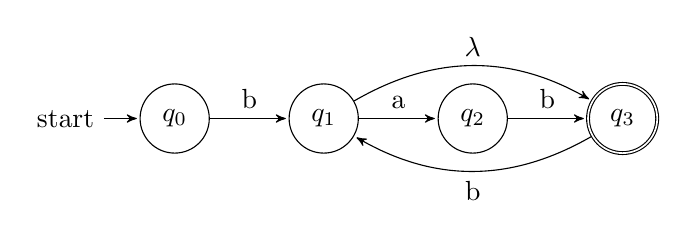
\begin{tikzpicture}[baseline=(q_0.north),>=stealth',shorten >=1pt, auto,node distance=1cm,align=center]
			\node[state,initial] (q_0) {$q_0$};
			\node[state] [right=of q_0] (q_1) {$q_{1}$};
			\node[state] [right=of q_1] (q_2) {$q_{2}$};
			\node[state,accepting] [right=of q_2] (q_3) {$q_{3}$};
			\path[->]
				(q_0) edge node {b} (q_1)
				(q_1) edge node {a} (q_2)
				(q_2) edge node {b} (q_3)
				(q_1) edge [bend left] node {$\lambda$} (q_3)
				(q_3) edge [bend left] node {b} (q_1);
		\end{tikzpicture}
		\\Where $q_{0}$ is the empty string $\lambda$, $q_{1}$ is $\{b,babb\}^{*}$, $q_{2}$ is $\{\text{$w\in L$ that end with an $a$}\}$, $q_{3}$ is ${b,bab}^{*}$.
		\item[(ii)]The conversion of the NFA to a DFA is given below.\\
		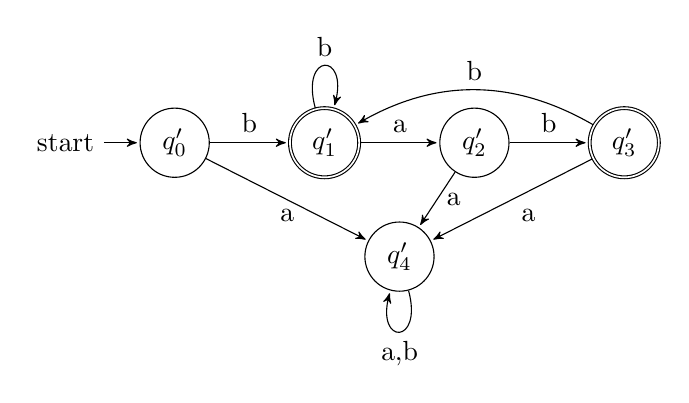
\begin{tikzpicture}[baseline=(q_0.north),>=stealth',shorten >=1pt, auto,node distance=1cm,align=center]
			\node[state,initial] (q_0) {$q_{0}^{\prime}$};
			\node[state,accepting] [right=of q_0] (q_1) {$q_{1}^{\prime}$};
			\node[state] [right=of q_1] (q_2) {$q_{2}^{\prime}$};
			\node[state,accepting] [right=of q_2] (q_3) {$q_{3}^{\prime}$};
			\node[state] [below=of $(q_1)!0.5!(q_2)$] (q_4) {$q_{4}^{\prime}$};
			\path[->]
				(q_0) edge node {b} (q_1)
				(q_1) edge [loop above] node {b} ()
				(q_1) edge node {a} (q_2)
				(q_2) edge node {b} (q_3)
				(q_3) edge [bend right] node [above] {b} (q_1)
				(q_0) edge node [below] {a} (q_4)
				(q_2) edge node [right] {a} (q_4)
				(q_3) edge node {a} (q_4)
				(q_4) edge [loop below] node {a,b} (); 
		\end{tikzpicture}
		\\Where $q_{0}^{\prime} = \{q_{0}\}$, $q_{1}^{\prime} = \{q_{1},q_{3}\}$, $q_{2}^{\prime} = \{q_{2}\}$, $q_{3}^{\prime} = \{q_{3}\}$ and $q_{4}^{\prime} = \emptyset$. States that are not denoted by prime are defined above in (a).
	\end{enumerate}
	\item[\textbf{(6)}]The steps to finding a regular expression for the NFA in Figure 2.38 are given below.\\
	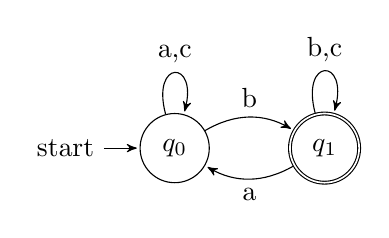
\begin{tikzpicture}[baseline=(q_0.north),>=stealth',shorten >=1pt, auto,node distance=1cm,align=center]
		\node[state,initial] (q_0) {$q_{0}$};
		\node[state,accepting] [right=of q_0] (q_1) {$q_{1}$};
		\path[->]
			(q_0) edge [loop above] node {a,c} ()
			(q_0) edge [bend left] node {b} (q_1)
			(q_1) edge [bend left] node {a} (q_0)
			(q_1) edge [loop above] node {b,c} ();
	\end{tikzpicture}\\
	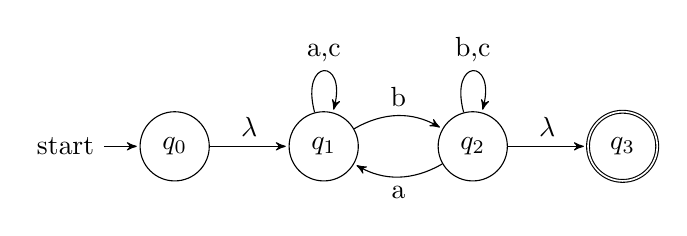
\begin{tikzpicture}[baseline=(q_0.north),>=stealth',shorten >=1pt, auto,node distance=1cm,align=center]
		\node[state,initial] (q_0) {$q_{0}$};
		\node[state] [right=of q_0] (q_1) {$q_{1}$};
		\node[state] [right=of q_1] (q_2) {$q_{2}$};
		\node[state,accepting] [right=of q_2] (q_3) {$q_{3}$};
		\path[->]
			(q_0) edge node {$\lambda$} (q_1)
			(q_1) edge [loop above] node {a,c} ()
			(q_1) edge [bend left] node {b} (q_2)
			(q_2) edge [bend left] node {a} (q_1)
			(q_2) edge [loop above] node {b,c} ()
			(q_2) edge node {$\lambda$} (q_3);
	\end{tikzpicture}\\
	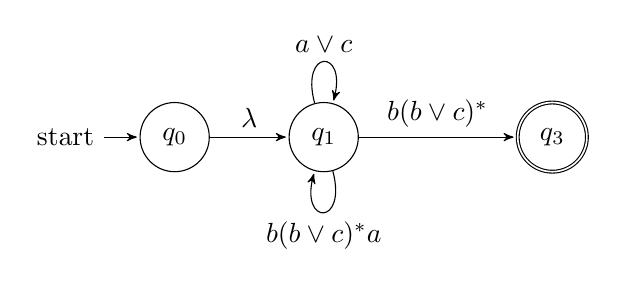
\begin{tikzpicture}[baseline=(q_0.north),>=stealth',shorten >=1pt, auto,node distance=1cm,align=center]
		\node[state,initial] (q_0) {$q_{0}$};
		\node[state] [right=of q_0] (q_1) {$q_{1}$};
		\node[state,accepting] [right=2cm of q_1] (q_2) {$q_{3}$};
		\path[->]
			(q_0) edge node {$\lambda$} (q_1)
			(q_1) edge [loop above] node {$a\lor c$} ()
			(q_1) edge node {$b(b\lor c)^{*}$} (q_2)
			(q_1) edge [loop below] node {$b(b\lor c)^{*}a$} ();
	\end{tikzpicture}\\
	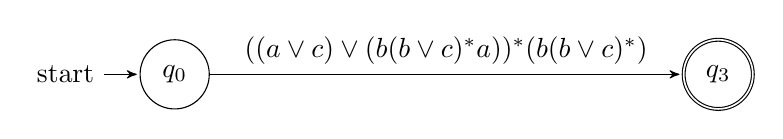
\begin{tikzpicture}[baseline=(q_0.north),>=stealth',shorten >=1pt, auto,node distance=1cm,align=center]
		\node[state,initial] (q_0) {$q_{0}$};
		\node[state,accepting] [right=6cm of q_0] (q_1) {$q_{3}$};
		\path[->]
			(q_0) edge node {$((a \lor c) \lor (b (b \lor c)^{*} a))^{*}(b (b \lor c)^{*})$} (q_1);
	\end{tikzpicture}\\
	Therefore, the regular expression for the language described by the NFA is $((a \lor c) \lor (b (b \lor c)^{*} a))^{*}(b (b \lor c)^{*})$.
	\item[\textbf{(7)}]Let Prefix($L$) = $\{u\:|\:\text{there is a string $v$ such that $uv \in L$}\}$. If $L$ is regular then there is a DFA, say $M$, that recognizes $L$. Now consider the DFA $M^{\prime}$ such that all states from which an accepting state is reachable in $M$ as accepting states for $M^{\prime}$. This DFA now recognizes Prefix($L$) since if $u$ is a prefix of $w$, meaning there is a string $v$ such that $uv = w$, and $w \in L$, then we must go over the letters of $u$ followed by the letters of $v$ to reach an accepting state in $M$. Thus, if there is a legal path that ends with an accepting state for $w$, we can create a DFA that identifies Prefix($L$) by making all states in the path leading to the accepting state for $w$ become accepting states. This then means that all prefixes of $w$ (i.e. $u$) is now recognized by the DFA $M^{\prime}$. $M^{\prime}$ is identical to $M$ for its alphabet $\Sigma$, set of states $Q$, starting state $q_{0}$ and transition function $\delta$, and the set of accepting states $F$ is defined as above. If we allow for $u$ to be $\lambda$, then we also keep that accepting states from $M$. Since there is a DFA $M^{\prime}$ that identifies Prefix($L$), Prefix($L$) is regular. Therefore, we conclude that if $L$ is regular then so is Prefix($L$).
\end{enumerate}

\end{document}